\chapter{Literature Review}\label{ch:lit_review}

\section{Background}

\subsection{History of the Smart Home}
The evolution of smart homes can be traced back to the early 1900s when the introduction of various electric household appliances promised to reduce the time spent on mundane household chores and free up more time for leisure, revolutionising domestic life.
Devices such as the electric mixer and iron, the world's first refrigerator in 1913, and the pop-up toaster in 1919, emerged in this period, bringing about the beginnings of a more automated home environment, with the following decades innovating accordingly~\cite{Hert16}.

In 1966, there was a significant leap forward in home automation technology when Jim Sutherland, an engineer from Pittsburgh, Pennsylvania created the ECHO IV.
The Electronic Computing Home Operator (ECHO IV) was the first device designed specifically for home automation and was hand-crafted with surplus electronic parts~\cite{Spic16}.
With the ability to compute shopping lists, control home temperature, limit children's television time with questionnaires and even tell the weather, this was the first glimpse at a whole-home computerised system that was capable of automating every element of home life.

The following year saw the introduction of Honeywell's Kitchen Computer.
A computer designed for housewives to use in the kitchen as a recipe storage device with a built-in chopping board.
At \$10,000 United States Dollars (USD) in 1967 (nearly \$100,000 USD today when accounting for inflation), this recipe storage device which had no display, was well described as ``amazingly beautiful and hopelessly impractical''~\cite{MANA23,Stei11,USIC}.
No units were ever sold.
Despite its failure on the open market, the device received a lot of attention and the public began to imagine a future where homes would be interactive.

Eight years later, in 1975, a group of engineers from Scotland released the X10 protocol.
Capable of controlling up to 256 devices on a single circuit, X10 sent messages to devices through a property's existing AC electrical wiring.
At the time, this was an efficient way to send basic signals through large spaces before the widespread adoption of wireless technology in all electronic devices.
It later advanced to be controllable from a computer, enabling users to schedule events and run decision-based sequences.
The protocol formed the basis for many domestic control installations for several decades and was one of the first protocols to completely cover the home automation spectrum, with power, security and lighting~\cite{X10}.

Throughout the 1980s and 1990s, the idea of having robots as companions was solidified in popular culture through science fiction movies.
During this same period, advancements in battery technology and the rapid decrease in the size of microprocessors meant that home robots became achievable, and by 1996, the Electrolux Trilobite was released, the world's first robot vacuum~\cite{Vacu}.
This class of device is now a quintessential smart home product and was a turning point for the industry.
The robot vacuum cleaner heralded the integration of the first wave of smart home devices that were not hard-wired into the building.
Along with this, the launch of the first-ever internet-connected refrigerator from LG, in the year 2000, demonstrated the increasing integration of technology into everyday household appliances~\cite{Maha17}.

This brings us to the current century, where, in the early 2000s, technology began to boom.
The home computer had become commonplace and the internet had become more accessible and understandable to the general public.
More smart devices, like speakers that speak to you about news headlines and weather or act as an alarm, began to appear on store shelves at affordable price points and home automation became a realistically achievable goal.

Today, smart homes are now a reality, they are not exclusively for the eccentric and wealthy.
They provide homeowners comfort, security, energy efficiency and convenience at all times, regardless of whether they are home or not.
Through the use of innovative technology, homeowners can turn their homes into state-of-the-art machines that can be controlled and monitored from anywhere in the world.

It is clear to see that with every iteration of the development of increasingly quasi-intelligent smart devices, early adopters were promised a more comfortable lifestyle with menial tasks being delegated to machines, saving more time for leisure.
With the beginnings of electric home appliances reducing the time required to dedicate to cooking and cleaning, through to interactive devices capable of holding simple conversations with users, this rapidly growing technology shows no signs of slowing down and its future capabilities are near limitless.

\subsection{Problems with Smart Homes}
With increasingly modernised smart home technology, its uses become more versatile, however, this has resulted in ever-growing challenges that hinder its expansive potential. Consequently, whilst many smart home technologies progress to solving existing problems, this allows for newer and more complex problems to point out existing flaws within their modus operandi.

There are several factors that limit the advancement of the industry and the effectiveness of smart devices as a whole.
Most of the problems with modern smart homes can be grouped into three main categories:
\begin{itemize}
    \item Interoperability
    \item Lack of true intelligence, and
    \item Requirement for Internet access
\end{itemize}
\cite{Wils15}.

\subsubsection{Interoperability}
There are many different competing standards in the world of smart homes, including devices that use Zigbee, Z-Wave, Bluetooth and Wi-Fi protocols.
This means that any given smart home device may not be compatible with another device, even if they are from the same manufacturer.
This can be frustrating for consumers who want to create a customised smart home environment that meets their specific needs and preferences when selecting their products and discourages their entry into the market.

There is currently a new protocol, called Matter, in development by the Connectivity Standards Alliance (CSA), in partnership with some of the leading smart home companies, that aims to unify each of these standards into a single, open-source standard and allow legacy devices to be able to communicate with one another.
This is a step in the right direction, however, considering historical context, this may result in it becoming an additional competing standard, with lengthy certification processes driving away smaller manufacturers, and, in turn, competition in the market.

Currently, there are many competing smart home platforms and hubs, such as Amazon Alexa, Google Home, Samsung SmartThings and Apple's HomeKit.
Even if the consumer does manage to choose devices all running on the same communication protocols, they may still be unable to control them all from a single app or interface.
Apple and Google are both notorious for having lengthy and expensive certification processes for third-party developers to integrate their devices into their platforms, which can be a significant barrier for smaller manufacturers, splintering the market further.

This usually leads to one of two possible outcomes for the consumer.
Either consumers end up locked into a single ecosystem, unable to switch to a different platform without replacing all of their devices, which can be a significant financial burden.
Or, they end up with a mix of devices from different manufacturers that are unable to communicate with one another each with its own dedicated app, which can be inconvenient and more time-consuming than not having smart devices at all.

\subsubsection{Lack of True Intelligence}
Despite their name, smart homes are not actually all that intelligent in their automation abilities.
Even in some of the most advanced smart homes, the devices are limited only to simple routines and schedules, and basic decision trees relying on primitive data from a limited number of sensors in the home.

With the recent advent of Artificial Intelligence (AI) and Machine Learning (ML) technologies, it is theoretically possible to create systems that can learn from user behaviour and adapt to their preferences.
However, most smart home devices are not yet capable of this level of predictive control and instead rely on the user to program them to perform specific tasks at specific times.

\subsubsection{Requirement for Internet Access}
Finally, the requirement for constant internet access for smart home devices may be one of the most significant inhibitors of the expansion of the smart home industry.
Many smart devices sold today often needlessly process all of their commands remotely, meaning that they require constant internet access to communicate with their respective cloud services in order to be able to control the devices, even from within your own home.
There are very few options on the market for devices that allow for local processing of commands.
For example, Google, Amazon and Apple's respective voice assistants, Google Assistant, Alexa and Siri, all require an internet connection to process voice commands, so without one, they are unable to control any devices in the home.

So if your internet connection goes down, you may be left with a house full of smart devices that are suddenly very dumb.
Not only will you not be able to access the devices remotely to control them or monitor your house, but you may also lose the ability to control them from within the same network as they cannot connect to their company's servers.

\section{Review of Existing Literature}

\subsection{Computer Vision for Smart Home Automation}
In a paper published at the 2019 International Conference on Communication and Signal Processing, Mohammad Hasnain R. et al. set out to ``develop a smart [Internet of Things] (IoT) based light control system'' using computer vision (CV) and artificial intelligence~\cite{Hasn19}.
Their objective was to reduce the wastage of electricity due to the ``negligence and forgetfulness'' of people using the environment~\cite{Hasn19}.

The authors correctly identify one of the biggest issues with presence detection in common home automation deployments.
Most setups use an array of infrared (IR) sensors to detect movement in a room but this poses a few challenges.
Firstly, any movement in view of the sensors will trigger an action that is intended only for human presence.
So if a book falls off a shelf or an animal runs past and interrupts the IR beams, then the sensor will report back a false positive result.
Additionally, another limitation of this method, which was not outlined in this paper, is that if a person remains stationary in the room, for example, whilst sitting on a couch, then there will be a false negative result suggesting that there is no human presence in the room.

To solve these downfalls of existing implementations, the authors took a different approach, utilising AI to identify people through a camera in a living space, enabling them to differentiate between objects and people.
However, there are a couple of areas that they did not explore that were within reach using the setup that they had implemented and that this thesis intends to expand upon.

A limitation regarding their investigation was that the authors only used the sensors as a toggle for LEDs with the aim of reducing unnecessary energy use.
Furthermore, to identify people in the camera, they used You only look once (Yolo), a computer vision AI model for used object detection, classification, and segmentation, which also has a built-in ``skeletonisation'' feature, allowing you to track a person's posture and make more intelligent decisions based on a person's movements.
These two ideas present an opportunity to fill a potential gap in the market making more intelligent decisions in the home using existing technology and real-world implementations.
Consequently, this thesis aims to implement a system capable of executing more complex tasks such as controlling other smart devices in the house like a television or blinds with more potential states than just off and on.

Aside from this paper, there has been extensive research into the use of computer vision in smart home deployments.
Nonetheless, very few of these discuss the integration of computer vision with smart home devices, and even fewer attempt to implement this integration.
There is extensive existing research that focuses on computer vision in homes, but it is mostly regarding intrusion detection and security~\cite{Cucc05,Garc17,Nand20,Patc15,Sefa14,Zhan19}.

V. Patchava et al. implemented a front-end for a smart home with the ability to toggle devices and stream the video feed from a camera with computer vision capabilities, while C. González García et al. implemented a system that could detect the presence of people and measured the rate of true positives, false positives, true negatives and false negatives~\cite{Patc15,Garc17}.
Others implemented presence detection with CV and were able to identify intruders and any weapon that they were carrying~\cite{Cucc05,Nand20}.
These papers discuss facial recognition software and the ability to alert homeowners of potential intruders.
Moreover, the authors discuss integration with custom smart home dashboards and IoT platforms, but do not discuss the integration of these systems with smart home devices and automation, which is the primary focus of this thesis.

\subsection{Human Action Recognition for Smart Home Automation}
Futher research exists into potential methods of person tracking, human action recognition and behaviour analysis using cameras in the home~\cite{Chaa13}.
Here, there is more of a focus on using this technology to support the elderly and the disabled, through ambient assisted living (AAL) to ``improv[e] their quality of life and [maintain] their independence''~\cite{Chaa13}.

A. Chaaraoui et al. discuss their deployment with both RGB cameras collecting information and recognising ``key poses'' and hand gestures by creating silhouettes of the person, and also by using RGB-D cameras using the depth information to more accurately track movements.
They were able to achieve this using a Microsoft Kinect camera and depth sensor ``with low-cost and real-time performance'', which is the same sensor that was used for preliminary testing in this thesis, as will be covered in more detail in Chapter~\ref{ch:project_prep}.
This existing deployment shows promising signs that the proposed setup should work smoothly in a home environment.
While they were able to get these systems working in real-time, recognising primitive human actions such as standing, walking, sitting and falling, there was no mention in the paper of actual integration with home devices.

In 2000, J. Krumm et al. followed very similar processes, using background subtraction to create silhouettes of people and overlaying depth data over the top of these cutouts through stereo images~\cite{Krum00}.
However, due to their early adoption of the technology they were somewhat limited by the computational power of computers during this period and had to run far more complicated and unwieldy setups that would not be suitable for a real home deployment today.
This meant that their trackers ran at only 3.5 Hz, even with the computational load shared between three computers, and often had trouble tracking more than three people at a time or people wearing similarly coloured clothing.

The authors were able to integrate their system with some home devices with custom programs such as a wireless mouse that could be carried to any table in the room and the clicks and movements of the mouse would be redirected to the nearest computer display.
Another program ``automatically start[ed] and stop[ped] a [Videocassette Recorder] (VCR) or [Digital Video Disc] (DVD) movie when a person sits on or stands up from a couch.''
The film would also be ``automatically rerouted to different displays in the room, depending on where the person [sat]''~\cite{Krum00}.

These are similar objectives to what this thesis partially aims to achieve, however, the technology has advanced significantly since then and the proposed setup should be able to run on a single computer with a single camera and depth sensor, making it more accessible to the general public.

\subsection{Gesture Recognition for Smart Home Automation}
In 2017, S. Desai and A. Desai proposed an algorithm for gesture recognition for home automation, also using the Microsoft Kinect~\cite{Desa17}.
Their proposal was specific to only recognising hand gestures, not full-body tracking.
This involved segmenting the hand from the image at a specified depth range of 250-650mm, removing the noise and background from the image and converting the RGB into a solid binary black and white image, as shown in Figure~\ref{fig:hand_gestures}.
The finger positions were then compared against a set of predefined gestures and then classified.
The classification then defines the action that the system should take, sending a signal to an Arduino board to control different home appliances such as a television, charger or fan.

\begin{figure}[!htb]
    \caption{Extracted Hand Gestures from Microsoft Kinect~\protect\cite{Desa17}}
    \centering
    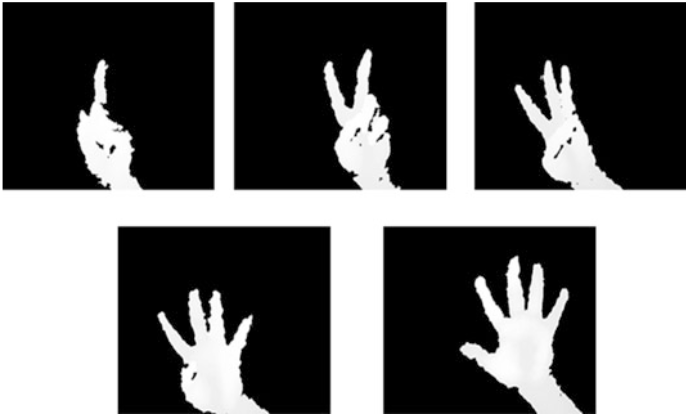
\includegraphics[width=0.6\textwidth]{Hand Gestures.png}
    \label{fig:hand_gestures}
\end{figure}

Using this technique, they were able to achieve an 88\% accuracy rate in recognising the gestures.
This is an insufficient accuracy rate for a real-world deployment, as users would have to repeat the gesture multiple times at least one in every 10 attempts in order to get the desired result.
Additionally, this only worked when users were giving gestures within 65cm from the camera, and only within a 40cm range.
This is not practical for day-to-day use as this would either require dozens of cameras per room, spread out every 1.3m, or it would require users to get up from wherever they are in the room and move to the camera in order to control their devices.
In this case, controlling their devices manually may be equally as convenient.
Due to these limitations, tracking gestures, only via hand movements, does not appear to be a viable solution for smart home automation, and full body tracking may be required to make this technology more practical for everyday use.

This paper, among others, refers also to computer vision technology recognising gestures through wearable devices~\cite{Krum00,Star00,Vole22}.
Implementing a system to track wearable devices opens up many possibilities for gesture recognition as well as the potential to integrate medical monitoring tools with it.
In fact, using the wearable device, T. Starner et al. were able to track the user's gestures against control gestures, which measure continuous input from the user, with an accuracy of 95\% and user-defined gestures with an accuracy of 97\%~\cite{Star00}.

Using a device that interacts directly with the user's body, will significantly increase the accuracy of gesture recognition, as the device is able to measure its own movements, and hence the user, as opposed to a potentially distant camera that attempts to infer the user's movements based on depth data.
However, this creates a significant hurdle as the user must be wearing the device at all times in order to control their devices, which significantly impedes the user experience and reduces the inconvenience that this technology is supposed to alleviate.

\subsection{Behaviour Monitoring for Elderly Care}
In a 2017 paper, ``A Behaviour Monitoring System (BMS) for Ambient Assisted Living,'' S. Eisa, and A. Moreira constructed an environment that could monitor the behaviour of elderly people in their homes~\cite{Eisa17}.
The system used passive infrared (PIR) sensors to monitor the movement of the elderly person between rooms and detect any deviations from their normal routine.
The theory behind their practice was that ``[a]n elderly person remains in good health as long as he or she can carry on his/her daily activities as usual with no significant deviations from the normal daily routine.''
This meant that if the system could identify any irregularities, then it could alert a carer or family member to check in on the user to ensure they are okay and potentially catch any health issues early.

This was implemented by treating the user's location in the house (by room) as a state machine, with the user able to transition states by moving between rooms, as shown in Figure~\ref{fig:state_machine}.
From this, a transition matrix is created for a given time of the day, which represents the probabilities of the user either staying in the same room or moving from one room to another.
Training an AI model to recognise the user's regular behaviour, the system could then recognise any deviations from this behaviour.
If the behaviour was deemed abnormal, it would then be classified to determine possible causes of the deviation, such as the user oversleeping if they are in their bedroom for too long, Table~\ref{tab:abnormal_behaviours} shows the abnormal behaviours that the authors listed.

\begin{figure}[!htb]
    \caption{Room-to-room State Transition Model~\protect\cite{Eisa17}.}
    \centering
    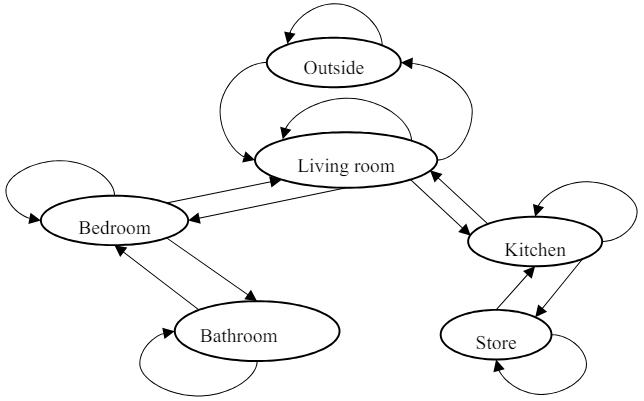
\includegraphics[width=\textwidth]{AAL State Machine.png}
    \label{fig:state_machine}
\end{figure}

\begin{table}[H]%!htb
    \caption{Abnormal Behaviours---Descriptions and related health-declines~\protect\cite{Eisa17}.}
    \centering
    \makebox[\textwidth][c] {
        \begin{tabular}{c c c}
            \hline
            \textbf{Behaviour} & \textbf{Description} & \textbf{Health-Declines} \\
            \hline
            OverSleeping &
            \begin{tabular}{@{}c@{}}
                An extended stay at bedroom;\\
                longer than usual.
            \end{tabular} &
            Mobility problems, strokes. \\
            \hline
            LessSleeping &
            \begin{tabular}{@{}c@{}}
                Detected motion at one of the rooms, not a \\
                bedroom, during the usual sleeping time.
            \end{tabular} &
            \begin{tabular}{@{}c@{}}
                Having sleepless time due to anxiety, \\
                depression or may be developing \\
                Alzheimer’s diseases.
            \end{tabular} \\
            \hline
            NotBackHome &
            \begin{tabular}{@{}c@{}}
                Monitored person stayed \\
                outside longer than usual.
            \end{tabular} &
            \begin{tabular}{@{}c@{}}
                Having trouble coming back home or get \\
                lost or wondering outdoors.
            \end{tabular} \\
            \hline
            Dead &
            \begin{tabular}{@{}c@{}}
                No movement and long stay at one of the \\
                rooms, not bedroom nor outside;
            \end{tabular} &
            Death. \\
            \hline
        \end{tabular}
    }
    \label{tab:abnormal_behaviours}
\end{table}

The model they implemented also self-updated once every week so that it could adapt to the user's ``behavioural changes that are not necessarily abnormal behaviours'' over time and account for seasonal changes in behaviour~\cite{Eisa17}.
This meant that they were able to implement a behaviour monitoring system that learned to adapt over time and consistently monitor the user's behaviour for any irregularities with primitive PIR sensors.
If this was achievable with such simple sensors, then the possibilities with more advanced depth sensors and computer vision should allow for more advanced behaviour monitoring and prediction.

There is also some overlap in this field with the computer vision and gesture recognition technologies that have been discussed.
M. Oudah et al. implemented a hand gesture recognition system, similar to that of S. Desai and A. Desai, but with the aim of assisting the elderly and disabled in their daily lives by allowing them to use gestures to get support if communication is a problem for them~\cite{Ouda21}.
With working deployments of both of these technologies in the AAL field, this shows promising signs for potential in the home automation field.

\section{Gaps in Literature}
After a thorough review of existing literature in the space that is being explored by this thesis, it is clear that there has been extensive research into many of the facets of the proposed system in consideration.
Computer vision is a widely researched field and has been applied to many different areas of smart home technology, from security to gesture recognition.
Human action recognition and gesture recognition have both also been studied for decades.

Despite this, there is a significant gap in the literature when it comes to the actual integration of these technologies with smart home devices and automation.
Most of the literature either discusses the technology in isolation or discusses implementation into smart homes on a theoretical level.
For example, there is vast research that discusses the use of computer vision for intrusion detection and security in a smart home, but the possibility of using this technology for automating tasks and controlling devices in the home is rarely considered. 
Almost none of the papers have actually implemented the technology into a real-world smart home environment and tested the results.
This presents a significant opportunity for this thesis to contribute to the field by providing a real-world implementation of these technologies and evaluating their performance and user experience.

There is also an opportunity to dive into a new area of research by combining these technologies with behaviour prediction to create a truly intelligent smart home environment.
Behaviour prediction and monitoring have been studied in the context of care for the elderly and disabled for ambient assisted living, but not in the context of smart home automation.
If done correctly, combining these technologies could allow for a smart home environment that can predict a user's behaviour and automate tasks in the home based on these predictions, without the need for user input.

\section{Problem Statement}
Smart homes today promise enhanced convenience, safety, and security through the connectivity of more and more devices and the automation of regular tasks.
However, several critical challenges prove to be a hindrance to their effectiveness as well as widespread adoption and, in turn, the growth of the industry.

Interoperability issues between devices and existing platforms, the lack of genuine intelligence in these automated systems, and the constant reliance on internet access pose significant obstacles to realising the true potential of smart home technology.

In an attempt to combat these challenges, this thesis aims to develop an entirely custom and customisable, intelligent environment where a user's movements will be able to accurately predict how to control devices within the home, through gesture recognition and behaviour prediction.
Utilising local processing and sensor data, the system will enhance convenience, safety, and security without relying on internet connectivity or support from third-party companies to allow interoperability.

Moreover, with several gaps in the existing research and literature in this area, this thesis aims to be able to integrate computer vision techniques and depth sensor technology into a smart home environment, utitlising this data to assist in automation, not just home monitoring and security.
This will provide a real-world implementation of these technologies and a live demonstration of the home's capabilities, as opposed to the theoretical implementations that are currently discussed in the recent literature.
The implementation of behavioural prediction technology, commonly used in AAL systems, will also be explored to predict user behaviour and automate tasks in the home based on the user's regular routines.

Overall, this research endeavours to contribute to the evolution of smart homes by introducing innovative approaches to enhance their intelligence and autonomy, ultimately improving the quality of life for users.

\section{Aims and Outcomes}
The research objectives of this thesis include designing and implementing artificial intelligence and computer vision for movement prediction and gesture control, integrating these into existing smart home infrastructure, and evaluating the performance and user experience of the environment.

With entirely locally processed data, the system will be able to control devices within the home without the need for internet connectivity, enhancing convenience, safety, and security for users.
Computer vision techniques will be used to identify users in the home and track their movements and gestures to control devices, while AI will be used to predict user behaviour and automate tasks in the home.

The anticipated outcomes of this research include advancements in smart home technology, improved user experiences, and insights into addressing the broader challenges in the field as outlined in the literature review.
While the research focuses on addressing specific aspects of smart home functionality, certain limitations, such as device compatibility and privacy concerns, will be acknowledged and considered throughout the study.
